\documentclass[11pt]{article}
\usepackage{fullpage,amsthm,amsfonts,amssymb,epsfig,amsmath,times,algorithm,algorithmic}
\usepackage[table,xcdraw]{xcolor}

\newtheoremstyle{indented-remark}
{}
{}
{\addtolength{\leftskip}{2.5em}}
{}
{\bfseries}
{:}
{.5em}
{}

\newtheoremstyle{indented-proof}
{}
{}
{\addtolength{\leftskip}{2.5em}}
{}
{\slshape}
{.}
{.5em}
{}

\theoremstyle{definition}
\newtheorem{theorem}{Theorem}
\newtheorem{lemma}{Lemma}
\newtheorem{corollary}{Corollary}
\newtheorem{observation}{Observation}
\newtheorem{definition}{Definition}

\theoremstyle{plain}
\newtheorem{claim}{Claim}

\theoremstyle{indented-remark}
\newtheorem{case}{Case}

\theoremstyle{indented-proof}
\newtheorem*{proofofcase}{Proof of Case}

\begin{document}

\begin{center}
{\bf\Large CMPS 102 --- Fall 2018 ---  Homework 2}
\end{center}

\begin{center}
\textit{"I have read and agree to the collaboration policy." - \textbf{Kevin Wang}}
\end{center}

\section*{Solution to Problem 1: Hadamard Matrix}

\begin{claim}
$H_{n} = \frac{1}{\sqrt{2}}
\begin{bmatrix} 
H_{n-1} & H_{n-1} \\
H_{n-1} & -H_{n-1} 
\end{bmatrix}$ where $H_{n}[i,j] = \frac{1}{\sqrt{2^{n}}}(-1)^{i \cdot j}$
\end{claim}

\begin{proof}
Given that $H_{n}[i,j] = \frac{1}{\sqrt{2^{n}}}(-1)^{i \cdot j}$, let matrix $H_{n} = \frac{1}{\sqrt{2^{n}}} H'_{n}$ where $H'_{n}[i,j] = (-1)^{i \cdot j}$. \newline
\noindent Let $A_{n}$, $B_{n}$, $C_{n}$, and $D_{n}$ be the four $2^{n-1} \times 2^{n-1}$ sized submatrices formed when dividing matrix $H_{n}$ into quarters as shown below:

\begin{minipage}{0.4\textwidth}
\begin{figure}[H]
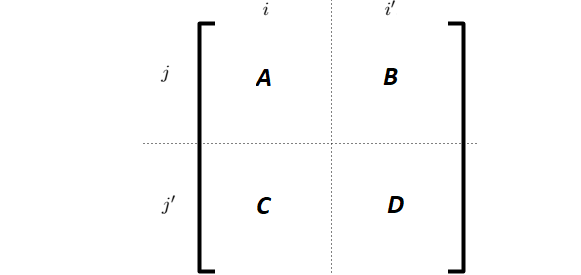
\includegraphics[scale=0.4]{images/MatrixQuadrants.png}
\end{figure}
\end{minipage} \hfill
\begin{minipage}{0.5\textwidth}
where $i,j \in [0, 2^{n-1})$ \newline
where $i',j' \in [2^{n-1}, 2^{n})$ \newline
\newline
Note that $i',j' = i,j + 2^{n-1}$, where\\
$2^{n-1}$ is the $n$-bit binary number consisting of the hi-order bit 1 followed by $(n-1)$ 0 bits.
\end{minipage} \newline

\noindent By definition of a Walsh-Hadamard matrix, the submatrix $A_{n}$ is constructed such that the $(i,j)$-th entry of 
$A_{n}[i,j] = \frac{1}{\sqrt{2^{n}}}(-1)^{i \cdot j}$ 
where $i,j \in [0, 2^{n-1})$. As such,
\begin{align}
A_{n}[i,j] &= \frac{1}{\sqrt{2^{n}}}H'_{n-1}[i,j]\notag \\
&= \frac{1}{\sqrt{2}} \times \frac{1}{\sqrt{2^{n-1}}}H'_{n-1}[i,j]\notag \\
\implies A_{n} &= \frac{1}{\sqrt{2}}H_{n-1}\notag
\end{align}

\noindent By definition of a Walsh-Hadamard matrix, the submatrix $B_{n}$ is constructed such that the $(i',j)$-th entry of 
$B_{n}[i',j] = \frac{1}{\sqrt{2^{n}}}(-1)^{i' \cdot j}$ where $i' = i + 2^{n-1}$. As such,
\begin{align}
i' \cdot j &= (i + 2^{n-1}) \cdot j\notag \\
&= (i \cdot j) + (2^{n-1} \cdot j)\notag \\
&= (i \cdot j) + [(1)(0) + (0)(j_{bit}) + (0)...]\notag \\
&= (i \cdot j) + 0\notag \\
\newline
B_{n}[i',j] &= \frac{1}{\sqrt{2^{n}}}H'_{n-1}[i',j]\notag \\
&= \frac{1}{\sqrt{2^{n}}}H'_{n-1}[i,j]\notag \\
&= \frac{1}{\sqrt{2}} \times \frac{1}{\sqrt{2^{n-1}}}H'_{n-1}[i,j]\notag \\
\implies B_{n} &= \frac{1}{\sqrt{2}}H_{n-1}\notag
\end{align}
\noindent We note that the vice versa $i,j'$ is an equivalent case. As such, 
$C_{n} = \frac{1}{\sqrt{2}}H_{n-1}$. \newline

\noindent Finally, by definition of a Walsh-Hadamard matrix, the submatrix $D_{n}$ is constructed such that the $(i',j')$-th entry of 
$D_{n}[i',j'] = \frac{1}{\sqrt{2^{n}}}(-1)^{i' \cdot j'}$ where $i',j' = i,j + 2^{n-1}$. 
As such,
\begin{align}
i' \cdot j' &= (i + 2^{n-1}) \cdot (j + 2^{n-1})\notag \\
&= (i \cdot (j + 2^{n-1})) + (2^{n-1} \cdot (j + 2^{n-1}))\notag \\
&= (i \cdot j) + (i \cdot 2^{n-1}) + (j \cdot 2^{n-1}) + (2^{n-1} \cdot 2^{n-1})\notag \\
&= (i \cdot j) + 2[(1)(0) + (0)(i,j_{bit}) + (0)...] + [(1)(1) + (0)(0) + ...]\notag \\
&= (i \cdot j) + (0) + (1)\notag \\
&= (i \cdot j) + 1\notag \\
\newline
D_{n}[i',j'] &= \frac{1}{\sqrt{2^{n}}}H'_{n-1}[i',j']\notag \\
&= \frac{1}{\sqrt{2^{n}}}[H'_{n-1}[i,j] \times (-1^{1})]\notag \\
&= - \frac{1}{\sqrt{2}} \times \frac{1}{\sqrt{2^{n-1}}}H'_{n-1}[i,j]\notag \\
\implies D_{n} &= - \frac{1}{\sqrt{2}}H_{n-1}\notag
\end{align}

\noindent Lastly, we piece the matrix together and get the recursive representation:
\begin{align}
H_{n} &=
\begin{bmatrix} 
A_{n} & B_{n} \\
C_{n} & D_{n} 
\end{bmatrix}\notag \\
&=
\begin{bmatrix} 
\frac{1}{\sqrt{2}}H_{n-1} & \frac{1}{\sqrt{2}}H_{n-1} \\
\frac{1}{\sqrt{2}}H_{n-1} & - \frac{1}{\sqrt{2}}H_{n-1} 
\end{bmatrix}\notag \\
&= \frac{1}{\sqrt{2}}
\begin{bmatrix} 
H_{n-1} & H_{n-1} \\
H_{n-1} & -H_{n-1} 
\end{bmatrix}\notag
\end{align}
\end{proof}

\newpage

\begin{claim}
The Euclidian norm of every column and every row is 1.
\end{claim}

\begin{proof}
Let matrix $H_{n} = \frac{1}{\sqrt{2^{n}}} H'_{n}$ where $H'_{n}[i,j] = (-1)^{i \cdot j}$. 
\newline

\noindent We define the Euclidian norm as the square root of the absolute squares of its elements. Because each element of $H_{n}$ is equal to $\frac{1}{\sqrt{2^{n}}} \times \pm 1$, the Euclidian norm of every column and row in the $2^{n} \times 2^{n}$ Walsh-Hadamard matrix $H_{n}$ is equal to:
\begin{align}
\| H_{n} \| &= \sqrt{\bigg( \pm \frac{1}{\sqrt{2^{n}}} \bigg) ^{2} \times 2^{n}}\notag \\
&= \sqrt{\frac{2^{n}}{2^{n}}}\notag \\
&= 1\notag
\end{align}
\end{proof}

\newpage

\begin{lemma}
Let $M$ be a matrix with size $2^{n} \times 2^{n}$ and let $M^{T}$ be its transpose. If $M$ is an orthonormal matrix, then $M^{T}M = I_{2^{n} \times 2^{n}}$.
\begin{proof}
The result of $M^{T}M$ is a matrix where $[i,j]$ is equal to the dot product of columns $i$ and $j$. As the dot product of every column must be 0 and each column has a Euclidian norm of 1, the result is the Identity matrix.
\end{proof}
\end{lemma}

\begin{claim}
The columns of $H_{n}$ form an orthonormal basis.
\end{claim}

\begin{proof}
Let $H_{n} = \frac{1}{\sqrt{2}}
\begin{bmatrix} 
H_{n-1} & H_{n-1} \\
H_{n-1} & -H_{n-1} 
\end{bmatrix}$ where $H_{n}[i,j] = \frac{1}{\sqrt{2^{n}}}(-1)^{i \cdot j}$. \newline 

\noindent Let $H^{T}_{n} = H_{n}$ due to the commutative property of the bitwise dot product $i \cdot j$. By Lemma 1, the base case $H_{1}$ is an orthonormal matrix:
\begin{align}
H_{1}^{T}H_{1} &= H_{1}H_{1} \notag \\
&= \frac{1}{\sqrt{2}}
\begin{bmatrix} 
1 & 1 \\
1 & -1 
\end{bmatrix}
\frac{1}{\sqrt{2}}
\begin{bmatrix} 
1 & 1 \\
1 & -1 
\end{bmatrix} \notag \\
&= \frac{1}{2}
\begin{bmatrix} 
1+1 & 1-1 \\
1-1 & 1+1 
\end{bmatrix}\notag \\
&= 
\begin{bmatrix} 
1 & 0 \\
0 & 1 
\end{bmatrix}\notag \\
&=
I_{2^{1} \times 2^{1}} \notag
\end{align}

\noindent Let us assume that $H_{n-1}$ is orthonormal: 
\begin{center}
$H_{n-1}^{T}H_{n-1} = H_{n-1}H_{n-1} = I_{2^{n-1} \times 2^{n-1}}$
\end{center}

\noindent Then:
\begin{align}
H_{n}^{T}H_{n} &= H_{n}H_{n} \notag \\
&= \frac{1}{\sqrt{2}}
\begin{bmatrix} 
H_{n-1} & H_{n-1} \\
H_{n-1} & -H_{n-1}  
\end{bmatrix}
\frac{1}{\sqrt{2}}
\begin{bmatrix} 
H_{n-1} & H_{n-1} \\
H_{n-1} & -H_{n-1} 
\end{bmatrix} \notag \\
&= \frac{1}{2}
\begin{bmatrix} 
(H_{n-1}H_{n-1})+(H_{n-1}H_{n-1}) & (H_{n-1}H_{n-1})-(H_{n-1}H_{n-1}) \\
(H_{n-1}H_{n-1})-(H_{n-1}H_{n-1}) & (H_{n-1}H_{n-1})+(H_{n-1}H_{n-1})
\end{bmatrix}\notag \\
&= 
\begin{bmatrix} 
H_{n-1}H_{n-1} & 0 \\
0 & H_{n-1}H_{n-1} 
\end{bmatrix}\notag \\
&=
\begin{bmatrix} 
I_{2^{n-1} \times 2^{n-1}} & 0 \\
0 & I_{2^{n-1} \times 2^{n-1}} 
\end{bmatrix}\notag \\
&=
I_{2^{n} \times 2^{n}} \notag
\end{align}
\end{proof}

\newpage

\noindent Let a vector $v \in \mathbb{R}^{2^{n}}$ and let 
$H_{n} = \frac{1}{\sqrt{2}}
\begin{bmatrix} 
H_{n-1} & H_{n-1} \\
H_{n-1} & -H_{n-1} 
\end{bmatrix}$
\begin{algorithm}
\caption{Uses divide-and-conquer to compute $H_{n} \cdot v$}
\begin{algorithmic}
\STATE \textbf{Hadamard-Vector-Product ($H_{n}$ , $v$ , $n$):}
\STATE Let $v_{1} = 
\begin{bmatrix} 
v_{0} \\
\vdots \\
v_{(m/2) -1} 
\end{bmatrix}$ and
$v_{2} = 
\begin{bmatrix} 
v_{m/2} \\
\vdots \\
v_{m-1} 
\end{bmatrix}$ ,
where $m = 2^{n}$
\STATE Let $H_{n} \cdot v =  
\begin{bmatrix} 
(H_{n} \cdot v)_{A} \\
(H_{n} \cdot v)_{B} 
\end{bmatrix}$, where
\begin{align}
(H_{n} \cdot v)_{A} &= H_{n-1} \cdot v_{A} + H_{n-1} \cdot v_{B} = H_{n-1} \cdot (v_{A}+v_{B}) \notag \\
(H_{n} \cdot v)_{B} &= H_{n-1} \cdot v_{A} - H_{n-1} \cdot v_{B} = H_{n-1} \cdot (v_{A}-v_{B}) \notag
\end{align}
\IF{$n = 1$}
\STATE Return $\frac{1}{\sqrt{2}}
\begin{bmatrix} 
H_{n} \cdot v_{A} \\
H_{n} \cdot v_{B} 
\end{bmatrix}$
\ELSE [$n > 1$]
\STATE Return $
\begin{bmatrix}
\text{Hadamard-Vector-Product } (H_{n-1} , (v_{A}+v_{B}) , n-1) \\
\text{Hadamard-Vector-Product } (H_{n-1} , (v_{A}-v_{B}) , n-1)
\end{bmatrix}$
\ENDIF
\end{algorithmic}
\end{algorithm}

\begin{claim}
The time complexity of the algorithm is $O(m \log m)$, where $m = 2^{n}$.
\end{claim}

\begin{proof}
Each half of $H_{n} \cdot v$ takes time $T\big( \frac{m}{2} \big)$. Each vector/matrix addition or subtraction takes time $O(m)$.
Therefore, the recurrence relation for the algorithm is defined as:
\begin{center}
$T(m) = 2T\big( \frac{m}{2} \big) + O(m)$
\end{center}
Thus, by Case 2 of the Master Theorem, the algorithm's time complexity is $O(m \log m)$.
\end{proof}

\end{document}

